% add my chapters
% 
% It is strongly recommended that you read documentations located at
%   http://code.google.com/p/xjtuthesis/wiki/Landing?tm=6
% in advance of your compilation if you have not read them before.
%
% This work may be distributed and/or modified under the
% conditions of the LaTeX Project Public License, either version 1.3
% of this license or (at your option) any later version.
% The latest version of this license is in
%   http://www.latex-project.org/lppl.txt
% and version 1.3 or later is part of all distributions of LaTeX
% version 2005/12/01 or later.
%
% This work has the LPPL maintenance status `maintained'.
% 
% The Current Maintainer of this work is Weisi Dai.
%

%\chapter{溶菌酶的提取、分离纯化实验的结果分析}
\chapter{Analysis of Results of lysozyme Extraction, Separation and Property Experiments}

\hypertarget{header-n0}{%
	\section{Dextran Gel G100 Filtration}\label{header-n0}}

\subsection{Results}

\begin{table}[!h]
	\centering
	\caption{Result of Dextran Gel G100 Filtration}
	\begin{tabular}{@{}lllll@{}}
	\toprule
	Protein & Amount in egg white & \(M_{r}\) & pI & Abundance
	in Chromatography\\
	\midrule
	Ovalbumin & 54\% & 45 kDa & 4.5 & ++\\
	Ovotransferrin & 12\% & 76.6 kDa & 6.06 & +\\
	Ovomucoid & 11\% & 38 kDA & 4.1 & +\\
	Lysozyme & 3.4\% & 14 kDa & \hl{10.7} & -\\
	\bottomrule
	\end{tabular}
\end{table}

In our \emph{Dextran Gel G100 Filtration}, two chromatography are
obtained. We first conduct a detection at the flow rate of 5 ml/min. But
only one sample peek was observed in this experiment. We then decrease
the flow rate to 0.5ml/min. Surprisingly, 2 peaks chromatography was
obtained. We refer to the articles for the protein ingredients in the
egg-proteins and get the sheet. As we can see, there are mainly 4 kinds of
proteins in the egg. Theoretically, they can easily tell from each other
due to the distinction in molecular weight. As we predict, there should
be two peaks in the chromatography graph, which suits our experimental
result.

\begin{figure}[!h]
	\centering
	\includegraphics[width=0.7\linewidth]{图片2.png}
	\caption{The flow curve of Dextran Gel G100 Filtration (5ml/min)}
	\label{fig:g1001}
\end{figure}

\begin{figure}[!h]
	\centering
	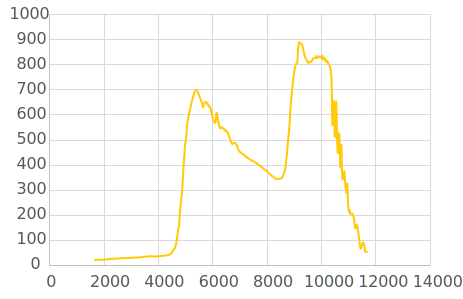
\includegraphics[width=0.7\linewidth]{图片1.png}
	\caption{The flow curve of Dextran Gel G100 Filtration (0.5ml/min), absorbance versus second}
	\label{fig:g1002}
\end{figure}

\subsection{Verification through SDS-PAGE}

The first SDS-PAGE was introduced after the \emph{G-100 Sephadex} size
exclusion chromatography. The result is listed as follows. There are
five different swim lanes from A1 to A5 in the graph, constructing a
concentration gradient. The chromatography shows that the main products
extracted from the solution located at 40-70 kDa while only little
product locates at \textasciitilde{}10 kDa, where lysozyme will be. We refer to the article to find out the reasons that may lead to the phenomena and find that the chromatography distribution of our examples is similar to the natural distribution of proteins in
eggs.

\begin{figure}[!h]
	\centering
	\includegraphics[width=0.7\linewidth]{图片3.png}
	\caption{Electrophoresis results of Dextran Gel G100 Filtration (compared with \citet{Liu2020})}
	\label{fig:g100}
\end{figure}

These facts convince us of the experimental failure and difficulties
using size exclusion chromatography to extract the lysozyme. Hence we
purchase the \emph{732 cation exchange resin} to conduct the further
experiment.

\section{Cation Exchange with Resin 732}

\subsection{Results}
We repeated this experiment on both a small column and a much bigger one. For simplicity, we abbrivate "concentrated elution peak from bigger column" to EPB and "concentrated elution peak from smaller column" to EPS.

During the elution, both of the scenerios showed only one peak.

\subsection{Verification through SDS-PAGE}

We made our second SDS-PAGE after the liquid chromatography and get really exciting results. There are three swim lanes in this PAGE-B1, B2 and B3. B2 is the commercial lysozyme product (2g/L) which we bought to examine the
resin as a standard product. B1,B3 is the concentrated solution extracted by the small column and big column, respectively. According to the result, all the examples located around
the 10-15kDa site, indicating the existence of lysozyme. \textbf{There is almost no other bands, indicating the thrilling purity of lysozyme.} We also notice
that the abundance of B1 and B3 are similar, which means the inspiring concentration of our extracted lysozyme.

\begin{figure}[!h]
	\centering
	\includegraphics[width=0.7\linewidth]{图片4.png}
	\caption{Electrophoresis results of Resin 732 Cation Exchange}
\end{figure}

\subsection{Summary on Two Types of Separation Methods}
\begin{figure}[!h]
	\centering
	\includegraphics[width=0.7\linewidth]{lyso.png}
	\caption{Composition of proteins in egg white \citep{Zhang2003}}
	\label{tab:compo}
\end{figure}

According to this chart (Fig. \ref{tab:compo}), we once believed that separation according to molecular weight might be successful. However, the first experimental design failed. The reason may be: the column is not long enough to separate all composites. We think the flow rate at 0.5 mL/min is not worthy to be decreased further, and no other factors matter if we don't change the filler. On the other side, Resin 732 helped us succeed because there is nearly no impurities at isoelectric point of more than 10 (the content of antibiotic protein is so low as to be ignored).


\section{Effect of pH on Enzyme Activity}

The absorbance curves, which were measured under identical condition, are shown in Fig \ref{fig:ph} and \ref{fig:ph89}. 
\begin{figure}[!h]
	\centering
	\includegraphics[width=0.9\linewidth]{figures/chp3_ph}
	\caption{Absorbance curves (pH=5,6,7)}
	\label{fig:ph}
\end{figure}

\begin{figure}[!h]
	\centering
	\begin{minipage}[c]{0.45\textwidth}
		\centering
		\includegraphics[width=\linewidth]{chp3_ph8}
	\end{minipage}
	\quad
	\begin{minipage}[c]{0.45\textwidth}
		\centering
		\includegraphics[width=\linewidth]{chp3_ph9}
	\end{minipage}
	\caption{Absorbance curves (pH=8,9)}
	\label{fig:ph89}
\end{figure}


Obviously, the lysozyme almost lose all its activity under pH 8 and 9. For the other three groups, we can roughly believe that the enzyme activity is highest when pH=5. However, we found in plenty of literature \citep{Yu-tong2006,Tian2012} that the optimal pH of lyzozyme is about 6. We also refered to some other groups of experiments, and found activity of lyzozyme when pH=6 is similar. 

This suggests that there might be some problem with the buffer (pH=6). Perhaps one of the reasons is that the pH test paper we used has low accuracy. Another problem is that enzyme activity should not be so low at pH 8 and 9. pH of egg white is about 8.0 and we used buffer whose pH is 9.0 to elute lysozyme from our column. Perhaps there is a shift in pH towards higher values when we were testing the activity, which could explain the optimal pH (5) might be larger and the activity problem. But this is not so possible. We believe we did not make such mistakes when configuring the buffers.

Unfortunately, we did not discover this fact at the time of experiment. So we go on to test enzyme activity when pH is tagged 6 (but may be 7 actually), which the literature indicated as an optimum.

\section{Enzyme Activity Calculation}

\begin{figure}[!h]
	\centering
	\includegraphics[width=0.9\linewidth]{figures/chp3_EPBcur}
	\includegraphics[width=0.9\linewidth]{figures/chp3_EPScur}
	\caption{Enzyme activity of the elution peaks}
	\label{fig:epbs}
\end{figure}

%\begin{figure}[!h]
%	\centering
%	\includegraphics[width=0.7\linewidth]{figures/chp3_EPScur}
%	\caption{a skecth of our polygon-sphere}
%	\label{fig:eps}
%\end{figure}

According to the definition mentioned in Sec. 2, we can calculate the enzyme activity of the concentrated solutions. We picked a linear region on the whole curve (See Fig \ref{fig:epbs}). The first few data points should be avoided because the mixture hasn't become homogenous and the reaction hasn't reached a steady state. We actually picked the 2nd minute, which means
\begin{gather*}
	EnzymeActivity=\dfrac{OD_{600}(120\mathrm{s})-OD_{600}(60\mathrm{s})}{0.5\mathrm{mL}}\times 10^{3}
\end{gather*}

The concentration we directly measured by the instrument is listed in Tab. \ref{tab:conc}:
\begin{table}[!h]
	\centering
	\caption{Concentration of concentrated enzyme solutions}
	\begin{tabular}{ccc}
		\toprule
		& {EPB (double dilution)} & {EPS EnzymeActivity} \\
		\midrule
		concentration $(\mathrm{g\cdot L^{-1}})$ & $3.725$  & $2.832$ \\
		\bottomrule
	\end{tabular}%
	\label{tab:conc}%
\end{table}%
which shows EPB was concentrated more times than EPS.

The activity results are listed in Tab. \ref{tab:res}:
\begin{table}[!h]
	\centering
	\caption{Enzyme Activity}
	\begin{tabular}{ccc}
		\toprule
		& {EPB (double dilution)} & {EPS (double dilution)} \\
		\midrule
		EnzymeActivity $(\mathrm{U\cdot mL^{-1}})$ & $50.0$  & $32.5$ \\
		SpecificActivity $(\mathrm{U\cdot mg^{-1}})$ & $13.4$ & $11.5$\\
		\bottomrule
	\end{tabular}%
	\label{tab:res}%
\end{table}%

Enzyme activities are of the same order of magnitude as that in the literature. 
There is no significant difference between the specific activities, which is a rational result.

Moreever, we also calculated the recovery rate of the bigger column roughly, but we did not record the exact loading volume.

\begin{table}[!h]
	\centering
	\caption{Recovery rate}
	\begin{tabular}{cc}
		\toprule
		& {EPB (double dilution)}\\
		\midrule
		Approximate loading volume/mL  & $6.5$ \\
		Recovery rate  & $92.4\%$ \\
		\bottomrule
	\end{tabular}%
	\label{tab:rec}%
\end{table}%

The result is also fascinating, which is probably due to a properly chosen elution pH.

\section{Reaction Kinetics Exploration}

In the previous sections, we have treated the absorbance curves as linear. But all curves seem to to plain as time passes, which means the reaction rate is decreasing slightly. As we used 2g/L standard enzyme when exploring the effect of pH, we believe it is likely that Machaelis-Menten equation doesn't apply here due to lower and lower substrate (bacteria) concentration. To better and fully describe the reaction, and to find indexes to measure enzyme activity without the influence of reactant concentrations, we explored the reaction kinetics.

We assume that substrate concentration is proportional to the absorbance, and tried many functions, and the results are listed in Tab \ref{tab:fit}. All are performed in Excel and MATLAB. Below the third horizontal line, there are several functions for which I cannot find actual meanings.

\begin{table}[!h]
	\centering
	\caption{Results of Fit}
	\begin{tabular}{ccccc}
		\toprule
		function & expression and data & pH=5 & pH=6 & pH=7 \\
		\midrule
		linear & $at+b$; 0-order reaction & 0.9717  & 0.9871  & 0.9667  \\
		MM as rate & $\int \mathrm{d}c/\mathrm{d}t=v\cdot c/(c+k_s)$ & unrational & unrational & 0.9944  \\
		MM as rate & same but without the first three points & 0.9574  & 0.9665  & 0.9545  \\
		MM as rate & $\int \mathrm{d}c/\mathrm{d}t=v\cdot c^2/(c+k_s)$ & 0.9842  & unrational & unrational \\
		exponential & $a\cdot \exp(bt)$; 1-order reaction & 0.9848  & 0.9791  & 0.9869  \\
		\midrule
		polynomial & $at^2+bt+c$ & 0.9968  & 0.9972  & 0.9981  \\
		\textbf{polynomial} & same but without the first three points & \textbf{0.9994}  & \textbf{0.9993}  & \textbf{0.9994} \\
		rational & $a/(t+b)$ & 0.9942  & 0.9961  & 0.9952  \\
		rational & $a/(t+b)+c$ & 0.9968  & 0.9965  & 0.9973  \\
		logistic & $a/(1+b\cdot \exp(ct))$ & 0.9832  & 0.9549  & 0.9840  \\
		\bottomrule
	\end{tabular}%
	\label{tab:fit}%
\end{table}%

We can see that:
\begin{itemize}
	\item
	Linear functions, which means the rate is constant, don't fit very
	well. Exponetial functions which imply the rate is proportional to
	substrate concentration, fit a bit better.
	\item
	If the rate complies with MM equation
	\[\dfrac{\mathrm{d}c}{\mathrm{d}t}=-v_m\cdot c/(c+k_s)\]
	we integrated it and failed to drive a meaningful result, because
	either \(R^2\) is low or \(K_s\) is negative or unrationally large.
	\item
	We also assume that when enzyme concentration is large, only part of
	the enzyme molecules bind to the substrate. The "effective" enzyme
	concentration is proportional to the substrate concentration. This can
	also be verified by modifying the derivation of MM equation. Thus
	\[\dfrac{\mathrm{d}c}{\mathrm{d}t}=-k_{cat}\cdot c^2/(c+k_s)\]
	However, this also failed because \(K_s\) is negative or too large,
	which leads that lower substrate concentration makes higher rate.
	\item
	The last three fits are just based on similar curve shape. We cannot
	explain them.
\end{itemize}

The most interesting one is polynomial fit, which fits best.
Especially when we delete the first three "unsteady-state" data points. However, it doesn't make sense. It is strange to have an chemical equation whose rate is proportional to reaction time. The integral of MM equation is a implicit function, so we don't have access to the terms and their meanings. This might be a problem waiting for mathematicians and chemists to solve.

The most rational explanation is, this quadratic function is a Taylor expansion (\eqref{tay}) of a more complex function or model that we haven't found out. 
\begin{equation}
	f(x)=f(x_0)+\dfrac{f^{\prime}(x_0)}{1!}(x-x_0)+\dfrac{f^{\prime \prime}(x_0)}{2!}(x-x_0)^2+\cdots \label{tay}
\end{equation}

We may divide $c_s=at^2+bt+c$ into:
\begin{itemize}
	\item constant $c$;
	\item linear part $bt$, which correspond to constant-rate reaction, like the early state of MM enzymatic reaction;
	\item nonlinear part $at^2$, which is the bias caused by some factors.
\end{itemize}

We think that $b$ decides the rate, or the enzyme activity. 

\begin{table}[!h]
	\centering
	\caption{Polynomial fit parameters}
	\begin{tabular}{cccc}
		\toprule
		parameters & pH=5  & pH=6  & pH=7 \\
		\midrule
		a     & 2.46e-06 & 1.20e-06 & 9.00e-07 \\
		b     & -1.86e-03 & -9.49e-04 & -1.10e-03 \\
		c     & 0.9788 & 0.9163 & 0.9537 \\
		\bottomrule
	\end{tabular}%
	\label{tab:para}%
\end{table}%

The results are not ideal too due to the pH problem. However, we propose this model to understand a nonlinear biological reaction curve like this. By analyzing the both parts, we may gain information about enzyme activity, reaction type, etc.


